\documentclass[12pt,a4paper]{article}

% ─── Page Layout ───────────────────────────────────────────────────────────────
\usepackage[a4paper, margin=0.8in, headheight=14pt]{geometry}

% ─── Fonts (XeLaTeX) ───────────────────────────────────────────────────────────
\usepackage{fontspec}
\usepackage{unicode-math}
\setmainfont{TeX Gyre Pagella}
\setmonofont[Scale=0.88]{TeX Gyre Cursor}
\setmathfont{Latin Modern Math}

% ─── Packages ──────────────────────────────────────────────────────────────────
\usepackage{xcolor}
\usepackage{colortbl}
\usepackage{titlesec}
\usepackage{enumitem}
\usepackage{tabularx}
\usepackage{longtable}
\usepackage{booktabs}
\usepackage{array}
\usepackage{amsmath}
\usepackage{tikz}
\usetikzlibrary{shapes.geometric, arrows.meta, positioning, calc, fit, decorations.pathreplacing, patterns}
\usepackage{tcolorbox}
\tcbuselibrary{skins, breakable}
\usepackage{hyperref}
\usepackage{fancyhdr}
\usepackage{graphicx}
\usepackage{microtype}
\hyphenpenalty=10000
\exhyphenpenalty=10000
\sloppy
\usepackage{caption}
\usepackage{setspace}
\usepackage{multirow}
\usepackage{tocloft}

% ─── Q&A helper ────────────────────────────────────────────────────────────────
\newcommand{\Q}[1]{\textbf{#1}\par\noindent\ignorespaces}

% ─── Colour Palette ────────────────────────────────────────────────────────────
\definecolor{myred}{RGB}{196,30,58}
\definecolor{mydark}{RGB}{30,30,50}
\definecolor{mygreen}{RGB}{14,120,80}
\definecolor{myteal}{RGB}{0,130,140}
\definecolor{myamber}{RGB}{180,100,0}
\definecolor{mypurple}{RGB}{100,30,160}
\definecolor{mygray}{RGB}{246,247,249}
\definecolor{mgframe}{RGB}{180,185,200}
\definecolor{watermark}{RGB}{145,150,170}
\definecolor{hdrred}{RGB}{250,232,235}
\definecolor{hdrgreen}{RGB}{220,244,233}
\definecolor{hdrteal}{RGB}{220,242,244}
\definecolor{hdramber}{RGB}{253,242,215}
\definecolor{hdrpurple}{RGB}{238,228,255}
\definecolor{hdrgray}{RGB}{238,240,245}

% ─── Section Formatting ────────────────────────────────────────────────────────
\titleformat{\section}
  {\large\bfseries\color{myred}}{\thesection.}{0.5em}{}
  [\vspace{1pt}{\color{myred}\rule{\linewidth}{0.8pt}}]
\titleformat{\subsection}
  {\normalsize\bfseries\color{myteal}}{\thesubsection}{0.5em}{}
\titlespacing*{\section}{0pt}{18pt}{7pt}
\titlespacing*{\subsection}{0pt}{11pt}{4pt}

% ─── Paragraph ─────────────────────────────────────────────────────────────────
\setlength{\parindent}{0pt}
\setlength{\parskip}{4pt}

% ─── TOC Styling ───────────────────────────────────────────────────────────────
\renewcommand{\cfttoctitlefont}{\large\bfseries\color{myred}}
\renewcommand{\cftaftertoctitle}{\par\noindent{\color{myred}\rule{\linewidth}{0.8pt}}}
\setlength{\cftbeforetoctitleskip}{0pt}
\setlength{\cftaftertoctitleskip}{6pt}
\renewcommand{\cftsecfont}{\normalsize\bfseries\color{mydark}}
\renewcommand{\cftsecpagefont}{\normalsize\bfseries\color{mydark}}
\renewcommand{\cftsecleader}{\cftdotfill{\cftdotsep}}
\setlength{\cftbeforesecskip}{7pt}
\renewcommand{\cftsubsecfont}{\small\color{mydark}}
\renewcommand{\cftsubsecpagefont}{\small\color{mydark}}
\setlength{\cftbeforesubsecskip}{3pt}
\setlength{\cftsubsecindent}{1.4em}

% ─── Table helpers ─────────────────────────────────────────────────────────────
\renewcommand{\arraystretch}{1.45}
\setlength{\tabcolsep}{6pt}
\arrayrulecolor{mydark}
\newcolumntype{B}[1]{>{\small\bfseries\raggedright\arraybackslash}m{#1}}
\newcolumntype{Y}{>{\small\raggedright\arraybackslash}X}
\renewcommand{\tabularxcolumn}[1]{m{#1}}

% ─── Header / Footer ───────────────────────────────────────────────────────────
\pagestyle{fancy}
\fancyhf{}
\fancyhead[L]{\small\color{myred}\textbf{ES-CS401}\;\color{mydark}--- Design and Analysis of Algorithms}
\fancyhead[R]{\small\color{myteal}\textbf{Module 4 Notes}}
\fancyfoot[C]{\small\color{mydark}\thepage}
\fancyfoot[R]{\small\color{watermark}\textit{\copyright\ Biraj Sarkar (CGEC)}}
\renewcommand{\headrulewidth}{0.5pt}
\renewcommand{\footrulewidth}{0.3pt}

% ─── Hyperref ──────────────────────────────────────────────────────────────────
\hypersetup{
  colorlinks=true, linkcolor=myteal, urlcolor=myteal,
  pdfauthor={Biraj Sarkar (CGEC)},
  pdftitle={ES-CS401 --- Module 4 Notes: Computability and NP-Completeness}
}

% ─── tcolorbox styles ──────────────────────────────────────────────────────────
\tcbset{
  tikzbox/.style={
    colback=mygray, colframe=mgframe, boxrule=0.6pt, arc=4pt,
    left=8pt, right=8pt, top=6pt, bottom=6pt,
    colbacktitle=mgframe, coltitle=mydark, fonttitle=\small\bfseries
  },
  defbox/.style={
    colback=hdrgreen, colframe=mygreen, boxrule=0.8pt, arc=4pt,
    left=9pt, right=9pt, top=6pt, bottom=6pt,
    colbacktitle=mygreen, coltitle=white, fonttitle=\small\bfseries
  },
  formulabox/.style={
    colback=hdrteal, colframe=myteal, boxrule=0.8pt, arc=4pt,
    left=9pt, right=9pt, top=7pt, bottom=7pt,
    colbacktitle=myteal, coltitle=white, fonttitle=\small\bfseries
  },
  examplebox/.style={
    colback=hdramber, colframe=myamber, boxrule=0.8pt, arc=4pt,
    left=9pt, right=9pt, top=6pt, bottom=6pt,
    colbacktitle=myamber, coltitle=white, fonttitle=\small\bfseries
  },
  masonbox/.style={
    colback=hdrpurple, colframe=mypurple, boxrule=0.8pt, arc=4pt,
    left=9pt, right=9pt, top=6pt, bottom=6pt,
    colbacktitle=mypurple, coltitle=white, fonttitle=\small\bfseries
  },
  exambox/.style={
    colback=hdrpurple, colframe=mypurple, boxrule=1pt, arc=5pt,
    left=10pt, right=10pt, top=8pt, bottom=8pt,
    colbacktitle=mypurple, coltitle=white, fonttitle=\bfseries,
    breakable, title after break={\textbf{Frequently Asked / Viva Questions (contd.)}}
  }
}
\tcbset{breakable}
\tcbset{after={\par\color{black}}}

% ─── TikZ styles ───────────────────────────────────────────────────────────────
\tikzset{
  block/.style={rectangle, draw=myteal, fill=hdrteal,
    text width=2.4cm, align=center, minimum height=0.95cm,
    font=\small, rounded corners=3pt, line width=0.7pt},
  redblock/.style={rectangle, draw=myred, fill=hdrred,
    text width=2.4cm, align=center, minimum height=0.95cm,
    font=\small, rounded corners=3pt, line width=0.7pt},
  amberblock/.style={rectangle, draw=myamber, fill=hdramber,
    text width=2.4cm, align=center, minimum height=0.95cm,
    font=\small, rounded corners=3pt, line width=0.7pt},
  sumjunc/.style={circle, draw=myamber, fill=hdramber,
    minimum size=0.62cm, font=\small, line width=0.8pt},
  arrow/.style={-Stealth, thick, color=mydark},
  redarrow/.style={-Stealth, thick, color=myred},
  line/.style={thick, color=mydark}
}

\begin{document}

% ─── Title Page ───────────────────────────────────────────────────────────────
\begin{center}
  {\LARGE\bfseries\color{myred} ES-CS401 --- Design and Analysis of Algorithms}\\[5pt]
  {\normalsize\color{mydark} Semester IV \quad$\bullet$\quad 3L:0T:0P \quad$\bullet$\quad 3 Credits}\\[3pt]
  {\normalsize\color{myteal}\textbf{Module 4 Exam Notes: Computability and NP-Completeness}}\\[3pt]
  {\small\color{mydark} CGEC \;$|$\; B.Tech ECE (2023--27) \;$|$\; \textit{Biraj Sarkar}}
\end{center}
\vspace{2pt}
\noindent{\color{myred}\rule{\linewidth}{1.5pt}}
\vspace{2pt}

\hypersetup{linkcolor=mydark}
\tableofcontents
\hypersetup{linkcolor=myteal}
\newpage

\section{Computability and NP-Completeness}
\subsection{Decision problems, computability and tractability}
\begin{tcolorbox}[defbox, title={Decision problem and decider}]
A \textbf{decision problem} asks a yes-or-no question. Its language is the set of encodings whose answer is yes. A \textbf{decider} halts on every input and gives the correct answer. A recogniser must accept yes instances, but may run forever on a no instance.
\end{tcolorbox}

\begin{itemize}[leftmargin=*, itemsep=3pt, topsep=4pt]
  \item \textbf{Search.} Produce a witness, such as a tour of cost at most $B$, if one exists.
  \item \textbf{Optimisation.} Find a solution of minimum cost or maximum value, such as the least-cost tour.
  \item \textbf{Decision.} Ask whether a solution meeting the bound $B$ exists. Define the certificate and its input encoding before assigning a complexity class.
  \item \textbf{Tractable.} In the usual complexity-theory convention, a decision problem is tractable if it can be solved in polynomial time. Constants and polynomial degree still matter in practice. A problem shown NP-hard is usually treated as computationally intractable unless $\mathrm{P}=\mathrm{NP}$.
\end{itemize}
TSP is decidable: exhaustive enumeration terminates even when it takes too much time for large instances. Undecidability is a different limitation. It rules out a decider altogether.
\begin{tcolorbox}[examplebox, title={Why the halting problem is undecidable}]
Suppose a program $H(P,x)$ always decides whether program $P$ halts on input $x$. Construct $D(P)$ that runs forever if $H(P,P)$ says yes, and halts if $H(P,P)$ says no. Run $D$ on its own encoding. If $H(D,D)$ says yes, $D(D)$ runs forever. If it says no, $D(D)$ halts. Either answer contradicts the specification, so no such $H$ exists.
\end{tcolorbox}

\subsection{Polynomial time and polynomial verification}
\begin{tcolorbox}[defbox, title={The classes P and NP}]
$\mathrm{P}$ contains decision problems solvable by a deterministic algorithm in polynomial time. $\mathrm{NP}$ contains decision problems for which every yes instance has a polynomial-length certificate that a deterministic polynomial-time verifier accepts. For a no instance, every proposed certificate must be rejected.
\end{tcolorbox}

\begin{tcolorbox}[formulabox, title={Formal verifier definition}]
A language $L$ is in $\mathrm{NP}$ if a polynomial $p$ and a polynomial-time verifier $V$ exist such that
\[
x\in L \iff \exists\, y,\quad |y|\le p(|x|)\ \text{and}\ V(x,y)=1.
\]
Equivalently, a nondeterministic machine can guess a certificate and verify it on an accepting computation branch within polynomial time.
\end{tcolorbox}

\begin{tcolorbox}[examplebox, title={Verifying the decision version of TSP}]
Given a proposed sequence of cities, check that it lists each city once, that the return edge is valid, and that the sum of weights does not exceed $B$. The certificate has polynomial length. The verifier uses polynomial time including the cost of arithmetic on the encoded weights.
\end{tcolorbox}

Every problem in $\mathrm{P}$ is in $\mathrm{NP}$ because a verifier can simply solve the decision problem. Whether $\mathrm{P}=\mathrm{NP}$ is open. The letters NP refer to nondeterministic polynomial time.

\section{Reductions and Completeness}
\subsection{Polynomial-time many-one reductions}
\begin{tcolorbox}[defbox, title={Polynomial-time reduction}]
For decision problems $A$ and $B$, write $A\le_p B$ when a polynomial-time function $f$ maps each instance of $A$ to an instance of $B$ with $x\in A$ exactly when $f(x)\in B$. Both yes and no answers must be preserved.
\end{tcolorbox}

\begin{tcolorbox}[tikzbox, title={Direction of a polynomial-time reduction}]
\centering
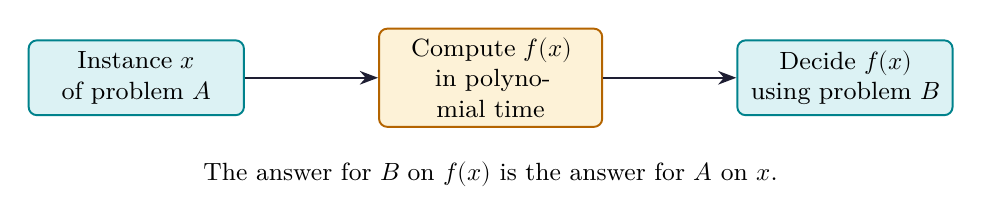
\begin{tikzpicture}[every node/.style={font=\small}]
\node[block,text width=2.5cm] (in) at (0,0) {Instance $x$\\of problem $A$};
\node[amberblock,text width=2.6cm] (f) at (4.5,0) {Compute $f(x)$\\in polynomial time};
\node[block,text width=2.5cm] (out) at (9,0) {Decide $f(x)$\\using problem $B$};
\draw[arrow] (in)--(f);
\draw[arrow] (f)--(out);
\node at (4.5,-1.22) {The answer for $B$ on $f(x)$ is the answer for $A$ on $x$.};
\end{tikzpicture}\par
\end{tcolorbox}

If $A\le_p B$ and $B\in\mathrm P$, then $A\in\mathrm P$: compute the transformation and run the solver for $B$. The output length of the transformation is polynomial because its runtime is polynomial. Composing two such transformations yields a polynomial-time reduction.
\begin{tcolorbox}[defbox, title={NP-hard and NP-complete}]
A problem $B$ is \textbf{NP-hard} if every problem in $\mathrm{NP}$ reduces to it in polynomial time. A decision problem is \textbf{NP-complete} if it is both NP-hard and in $\mathrm{NP}$. NP-hardness on its own supplies no certificate bound. Optimisation problems are commonly called NP-hard when solving them also solves an NP-hard decision version.
\end{tcolorbox}

\begin{enumerate}[leftmargin=*, itemsep=3pt, topsep=4pt]
  \item \textbf{Membership.} Identify a polynomial-length certificate for the target $B$ and give a polynomial-time verifier.
  \item \textbf{Known hardness.} Select an already NP-complete decision problem $A$ with a structure that maps naturally to $B$.
  \item \textbf{Construction.} Map each input $x$ of $A$ to $f(x)$ of $B$. Show that both building time and encoded output size are polynomial.
  \item \textbf{Equivalence.} Prove $x\in A\Rightarrow f(x)\in B$ and the reverse implication separately.
  \item \textbf{Conclusion.} Use transitivity to conclude that $B$ is NP-hard, then add membership to obtain NP-completeness.
\end{enumerate}
\begin{tcolorbox}[masonbox, title={Check the reduction direction}]
Reducing the target to a known NP-complete problem gives an upper bound in terms of that problem. To prove the target hard, reduce the known hard problem \emph{to the target}.
\end{tcolorbox}

\subsection{Cook's theorem: SAT is NP-complete}
\begin{tcolorbox}[defbox, title={SAT, CNF-SAT and 3-SAT}]
SAT asks if some assignment makes a Boolean formula true. CNF-SAT restricts the formula to an AND of clauses, each of which is an OR of literals. A literal is a variable or its negation. In 3-SAT each clause has at most three literals. The conventional exactly-three version can be obtained by padding shorter clauses.
\end{tcolorbox}

\textbf{Cook--Levin theorem.} SAT is NP-complete in the modern polynomial many-one formulation. To show membership in NP, use a truth assignment as the certificate and evaluate the formula. For NP-hardness, let a nondeterministic machine decide some $L\in\mathrm{NP}$ in time $T=p(n)$ on input $x$.
\begin{enumerate}[leftmargin=*, itemsep=3pt, topsep=4pt]
  \item \textbf{Represent the history.} Any accepting run fits in $T+1$ time rows and $O(T)$ tape positions, with one encoded tape symbol per cell and state/head information. The finite machine alphabet and state set are fixed.
  \item \textbf{Initial configuration.} Add clauses requiring the first row to encode the input, initial state, head position and blank remainder.
  \item \textbf{Legal transitions.} Use constraints between successive rows for the machine's step rule. Each step uses one consistent legal nondeterministic choice, updates the head neighbourhood and leaves untouched cells unchanged.
  \item \textbf{Acceptance.} Require an accepting configuration within the time bound. An accepting run can be padded by giving its accepting state an idle self-loop.
  \item \textbf{Equivalence and size.} A legal accepting run satisfies the clauses. A satisfying assignment decodes to a legal accepting run. The tableau and its transition constraints have polynomial size, so the construction is a polynomial-time reduction.
\end{enumerate}
\begin{tcolorbox}[examplebox, title={Splitting a long CNF clause}]
Use a fresh variable $z$ to replace $(a\lor b\lor c\lor d)$ by
\[
(a\lor b\lor z)\land(\neg z\lor c\lor d).
\]
If $a\lor b$ is true, choose $z$ false. If only $c\lor d$ is true, choose $z$ true. If all original literals are false, the two clauses demand both $z$ and $\neg z$. A chain of fresh variables splits longer clauses in linear size, preserving satisfiability.
\end{tcolorbox}

\textbf{Reading.} Stephen A. Cook, \href{https://www.cs.cmu.edu/~15455/resources/Cook1971-complx-thm-proof.pdf}{The Complexity of Theorem-Proving Procedures (1971)}. The paper uses oracle reducibility in its original formulation. The tableau argument above is presented in the modern SAT formulation used in exams.

\section{Standard NP-Complete Problems and Reductions}
\subsection{Decision formulations and certificates}
\par\vspace{5pt}
\begingroup
\setlength{\extrarowheight}{1pt}
\noindent\begin{tabularx}{\linewidth}{|B{3.4cm}|Y|Y|}
\hline
\textbf{Problem} & \textbf{Decision question} & \textbf{Certificate to verify} \\ \hline
3-SAT & Does this 3-CNF formula have a satisfying assignment? & Boolean values for the variables. \\ \hline
Clique & Is there a pairwise adjacent set of at least $k$ vertices? & A set of $k$ vertices and all their pair adjacencies. \\ \hline
Independent Set & Is there a set of at least $k$ pairwise non-adjacent vertices? & A set of $k$ vertices. No selected pair may share an edge. \\ \hline
Vertex Cover & Is there a set of at most $k$ vertices touching every edge? & A set of selected vertices. Check every edge endpoint pair. \\ \hline
Hamiltonian Cycle & Does a graph contain a cycle visiting every vertex once? & The cyclic vertex order and all required edges. \\ \hline
Decision TSP & Is some tour's total weight at most $B$? & A tour and its verified total cost. \\ \hline
Subset Sum & Can some subset of the input integers sum exactly to $B$? & An inclusion bit for each input item. \\ \hline
Decision Knapsack & Can selected items fit weight $W$ and attain value at least $K$? & An inclusion bit for each item. Verify both totals. \\ \hline
\end{tabularx}\par
\endgroup
The cited decision problems are standard NP-complete versions with their usual unrestricted inputs. Restricted cases may have faster algorithms. For example, Hamiltonian cycle is about visiting vertices once, whereas Eulerian cycle uses each edge once and has a polynomial-time test.

\subsection{Reduction from 3-SAT to Clique}
\begin{tcolorbox}[examplebox, title={Literal-occurrence graph}]
Let the 3-CNF input have $m$ clauses.
\begin{enumerate}[leftmargin=*, itemsep=3pt, topsep=4pt]
  \item Make one vertex per literal occurrence and mark its clause. Put no edge within a clause.
  \item Between different clauses, put an edge when the two literals are compatible, meaning neither is the negation of the other.
  \item Ask whether the graph has a clique of size $m$. There are at most $3m$ vertices and $O(m^2)$ edges.
\end{enumerate}
\textbf{Forward direction.} A satisfying assignment makes some literal true in each clause. Choose one true occurrence from each. True literals cannot contradict each other, so the chosen vertices form a clique.
\par
\textbf{Reverse direction.} An $m$-clique contains at most one vertex per clause, so it contains one from each. Its literals are pairwise compatible. Assign them true and choose the remaining variables arbitrarily. Each clause is satisfied.
\par
For $(x\lor y\lor\neg z)\land(\neg x\lor z\lor y)\land(x\lor\neg y\lor z)$, choose occurrences $x$, $y$ and $x$ from the three clauses. The occurrence of $x$ in each clause is a separate vertex. Setting $x$ and $y$ true satisfies the formula.
\end{tcolorbox}

\subsection{Graph complements and the cover relationship}
A set $S$ is a clique in $G$ exactly when it is independent in the complement $\overline G$. Also, $S$ is independent in a graph $H$ exactly when $V(H)\setminus S$ covers all edges. The latter equivalence holds because an uncovered edge would have both endpoints in $S$. Thus
\[
(G,k)_{\mathrm{Clique}}\mapsto
(\overline G,|V|-k)_{\mathrm{Vertex\ Cover}}
\]
preserves answers and is polynomial to construct.

\subsection{Hamiltonian Cycle to TSP and Subset Sum to Knapsack}
\begin{tcolorbox}[examplebox, title={TSP with costs 1 and 2}]
\begin{enumerate}[leftmargin=*, itemsep=2pt]
  \item \textbf{Build.} On the same $n\ge3$ vertices, build a complete weighted graph. Give original edges cost $1$ and nonedges cost $2$. Set the tour budget to $n$.
  \item \textbf{Forward direction.} A Hamiltonian cycle from the original graph uses $n$ cost-$1$ edges, so the budget is met.
  \item \textbf{Reverse direction.} Every tour uses $n$ edges. Any cost-$2$ edge makes the sum exceed $n$, so a tour meeting the budget uses original edges throughout.
\end{enumerate}
The construction has polynomial size and obeys the triangle inequality.
\end{tcolorbox}

\begin{tcolorbox}[examplebox, title={Decision Knapsack from Subset Sum}]
Given positive integers $a_i$ and target $B$, define item $i$ to have $w_i=v_i=a_i$ and choose $W=K=B$. A subset summing to $B$ is feasible and attains the value threshold. A feasible selection reaching the threshold has the same weight and value, so its sum is forced to equal $B$. The transformation copies only polynomially many bits.
\end{tcolorbox}

\begin{tcolorbox}[masonbox, title={What completeness lets you conclude}]
A polynomial-time algorithm for one NP-complete problem would imply $\mathrm{P}=\mathrm{NP}$. Completeness alone does not prove an exponential time lower bound, rule out useful exact algorithms on small cases, or prevent approximation. Undecidable problems can be NP-hard without being in NP. For example, a SAT instance can be encoded into a program that halts exactly when exhaustive assignment enumeration finds a satisfying assignment.
\end{tcolorbox}

\subsection{Why Subset Sum is NP-complete}
The certificate is the chosen subset. To prove hardness, reduce 3-SAT to Subset Sum using base-ten digit columns. For a formula with $n$ variables and $m$ clauses, reserve $n$ variable columns and $m$ clause columns.
\begin{enumerate}[leftmargin=*, itemsep=3pt]
  \item Give each variable two numbers, one for each truth value. Both have digit 1 in that variable's column and 0 in the other variable columns. In a clause column, the digit counts literals made true by that choice.
  \item Give each clause two additional numbers, with digits 1 and 2 in just its own clause column. They can add a total from 0 through 3 to that column.
  \item Set the target to digit 1 in every variable column and digit 4 in every clause column. There is no carry. Even selecting all available numbers contributes at most 2 to a variable column, and at most $3+1+2=6$ to a clause column.
\end{enumerate}
The variable columns force exactly one choice per variable. A clause receives $q$ satisfied literals, with $0\le q\le3$. The extra numbers can achieve target 4 exactly when $q\ge1$. Consequently the formula is satisfiable exactly when the digit target can be formed. There are $2n+2m$ numbers and their binary encodings each have $O(n+m)$ bits.
\begin{tcolorbox}[examplebox, title={Digit reduction for two variables and two clauses}]
For $(x\lor y)\land(\neg x\lor y)$, use columns $(x,y,C_1,C_2)$. The choices for $x$ are $1010$ and $1001$, and those for $y$ are $0111$ and $0100$. The target is $1144$. Picking both true gives $1010+0111=1121$. Add $0020$, $0001$ and $0002$ to obtain $1144$. The extra numbers merely complete clause counts after truth choices have satisfied the clauses.
\end{tcolorbox}

\newpage
\begin{center}
  {\large\bfseries\color{myred} Quick Revision --- Module 4}\\[3pt]
  {\small\color{mydark} Computability and NP-Completeness $|$ ES-CS401}
\end{center}
\noindent{\color{myred}\rule{\linewidth}{1.2pt}}\par\vspace{4pt}

\begin{tcolorbox}[formulabox, title={Key Concepts at a Glance}]
\renewcommand{\arraystretch}{1.35}
\noindent\begin{tabularx}{\linewidth}{B{4.5cm}Y}
Verifier & $x\in L$ iff some polynomial-length $y$ is accepted by a polynomial-time verifier. \\[3pt]
Reduction & $x\in A\iff f(x)\in B$ for $A\le_p B$. \\[3pt]
NP-complete & $\mathrm{NP}$ membership plus NP-hardness. \\[3pt]
Standard starting points & SAT, 3-SAT, Clique, Vertex Cover, Hamiltonian Cycle and Subset Sum. \\[3pt]
\end{tabularx}\par
\end{tcolorbox}

\begin{tcolorbox}[defbox, title={One-Line Definitions}]
\begin{itemize}[leftmargin=*, itemsep=3pt, topsep=4pt]
  \item \textbf{Decidable.} A program halts with the correct yes-or-no answer on every input.
  \item \textbf{Certificate.} An encoded witness presented to a verifier.
  \item \textbf{Clique.} A set of pairwise adjacent vertices.
  \item \textbf{Vertex cover.} A set touching every edge.
\end{itemize}
\end{tcolorbox}

\begin{tcolorbox}[exambox, title={Frequently Asked / Viva Questions}]
\begin{enumerate}[topsep=0pt, label=\textbf{Q\arabic*.}, itemsep=5pt, leftmargin=*]
  \item \Q{What is the distinction between a decider and a recogniser?}
    A decider halts on every input. A recogniser is allowed to loop on a no input.
  \item \Q{What does tractable mean in this context?}
    A deterministic polynomial-time decision algorithm exists.
  \item \Q{Why is every P problem in NP?}
    The verifier can ignore its witness and solve the decision problem.
  \item \Q{Is P equal to NP?}
    This remains an open problem.
  \item \Q{What must a polynomial-time reduction preserve?}
    Every source yes instance maps to a target yes instance, and every source no instance maps to a target no instance.
  \item \Q{Which way do you reduce to prove hardness?}
    From a known NP-complete decision problem to the target.
  \item \Q{What does Cook's theorem establish?}
    Boolean satisfiability is NP-complete.
  \item \Q{What is a tableau used for?}
    It encodes a polynomially bounded computation history using Boolean constraints.
  \item \Q{Why are two vertices in the same clause never adjacent in the 3-SAT to Clique reduction?}
    A clique of the desired size must choose one occurrence per clause.
  \item \Q{Why does cost at most n enforce a Hamiltonian cycle in the 1--2 TSP reduction?}
    Each of the n tour edges costs at least one. Any added cost-two edge exceeds the budget.
  \item \Q{Does NP-hardness guarantee an efficient verifier?}
    Only membership in NP gives the polynomial certificate guarantee.
\end{enumerate}
\end{tcolorbox}

\begin{tcolorbox}[tikzbox, title={Summary Comparison}]
\par\vspace{5pt}
\begingroup
\setlength{\extrarowheight}{1pt}
\noindent\begin{tabularx}{\linewidth}{|B{3.45cm}|Y|Y|}
\hline
\textbf{Class} & \textbf{Condition} & \textbf{Example} \\ \hline
P & Polynomial-time decision algorithm. & Graph reachability. \\ \hline
NP & Polynomial-length, polynomial-time-checkable yes certificates. & Reachability and SAT. \\ \hline
NP-complete & In NP and at least as hard as every NP problem. & SAT, 3-SAT and Clique. \\ \hline
NP-hard & All NP decisions reduce to it. & TSP optimisation under the usual decision-to-optimisation interpretation. \\ \hline
\end{tabularx}\par
\endgroup
\end{tcolorbox}

\end{document}
